% tests.tex
% $Header: tests.tex,v 0.1$

\section{Standalone Pelagic}\label{sec:standalonepel}
\subsection{Configuration}
\subsubsection{IFORT}
\begin{tabular}{|c|c|}
\hline
\hline
\rowcolor{LightCyan}
{\bf OPTION}   & {\bf VALUE} \\
\hline    
NAME     & test\_STD\_PEL \\
\hline       
ACTIVE   & A \\
\hline       
PRESET   & STANDALONE\_PELAGIC \\
\hline        
RUN      & bsub \\
\hline        
PROC     & '' \\
\hline    
ARCH     & ifort.inc \\
\hline    
RUNEXE   & '' \\
\hline    
PAREXE   & '' \\
\hline    
QUEUE    & '' \\
\hline    
PRECMD   & module load HDF5/hdf5-1.8.11\_parallel \\
         & NETCDF/netcdf-4.3\_parallel \\
         & NETCDF/parallel-netcdf-1.3.1 \\
\hline    
FORCING  & '' \\
\hline    
PRERUN   & '' \\
\hline    
COMPARE  & '' \\
\hline    
VALGRIND & '' \\
\hline    
\end{tabular}


\subsubsection{GFORTRAN}
\begin{tabular}{|c|c|}
\hline
\hline
\rowcolor{LightCyan}
{\bf OPTION}   & {\bf VALUE} \\
\hline    
NAME     & test\_STD\_PEL\_C \\
\hline    
ACTIVE   & A \\
\hline    
PRESET   & STANDALONE\_PELAGIC \\
\hline    
RUN      & bsub \\       
\hline    
PROC     & '' \\
\hline    
ARCH     & gfortran\_debug.inc \\
\hline    
RUNEXE   & '' \\
\hline    
PAREXE   & '' \\
\hline    
QUEUE    & '' \\
\hline    
PRECMD   & module load HDF5/hdf5-1.8.11\_parallel \\
         & NETCDF/netcdf-4.3\_parallel \\
         & NETCDF/parallel-netcdf-1.3.1 \\
\hline    
FORCING  & '' \\
\hline    
PRERUN   & '' \\
\hline    
COMPARE  & '' \\
\hline    
VALGRIND & '' \\
\hline        
\end{tabular}


\subsubsection{VALGRIND}
\begin{tabular}{|c|c|}
\hline
\hline
\rowcolor{LightCyan}
{\bf OPTION}   & {\bf VALUE} \\
\hline        
NAME     & test\_STD\_PEL\_M \\
\hline        
ACTIVE   & A \\
\hline        
PRESET   & STANDALONE\_PELAGIC \\
\hline    
RUN      & bsub \\
\hline    
PROC     & '' \\
\hline    
ARCH     & gfortran\_debug.inc \\
\hline        
RUNEXE   & '' \\
\hline        
PAREXE   & '' \\
\hline        
QUEUE    & '' \\
\hline        
PRECMD   & export NETCDF=/users/home/ans040/local; \\
         & export LD\_LIBRARY\_PATH=/users/home/ans040/local/lib:\$LD\_LIBRARY\_PATH \\
\hline        
FORCING  & '' \\
\hline        
PRERUN   & '' \\
\hline        
COMPARE  & '/users/home/ans040/dev/repo/bfm/tools/bfm\_test/tmp/test\_STD\_PEL' \\
\hline        
VALGRIND & valgrind --tool=massif --run-libc-freeres=no --stacks=yes \\
\hline        
\end{tabular}


\subsection{Result}
\begin{figure*}
  \centering
  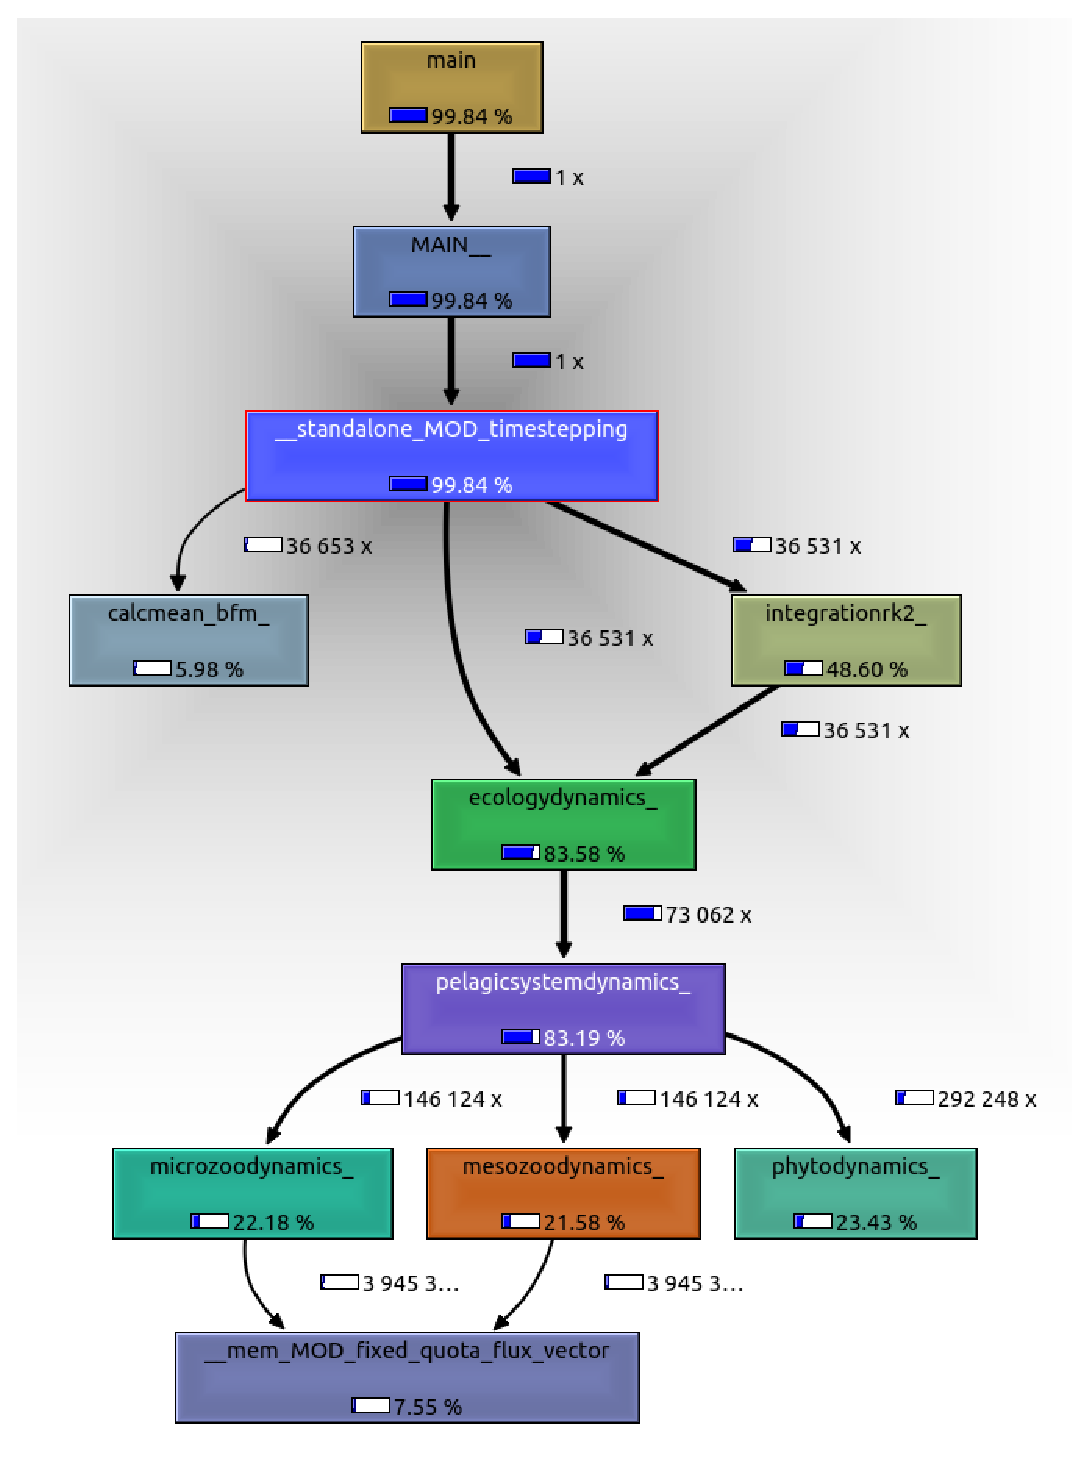
\includegraphics[width=\textwidth]{img/callgrind_std}
  \caption{Standalone Pelagic Call Graph}
  \label{fig:callgrind_std}
\end{figure*}

\begin{figure*}
  \centering
  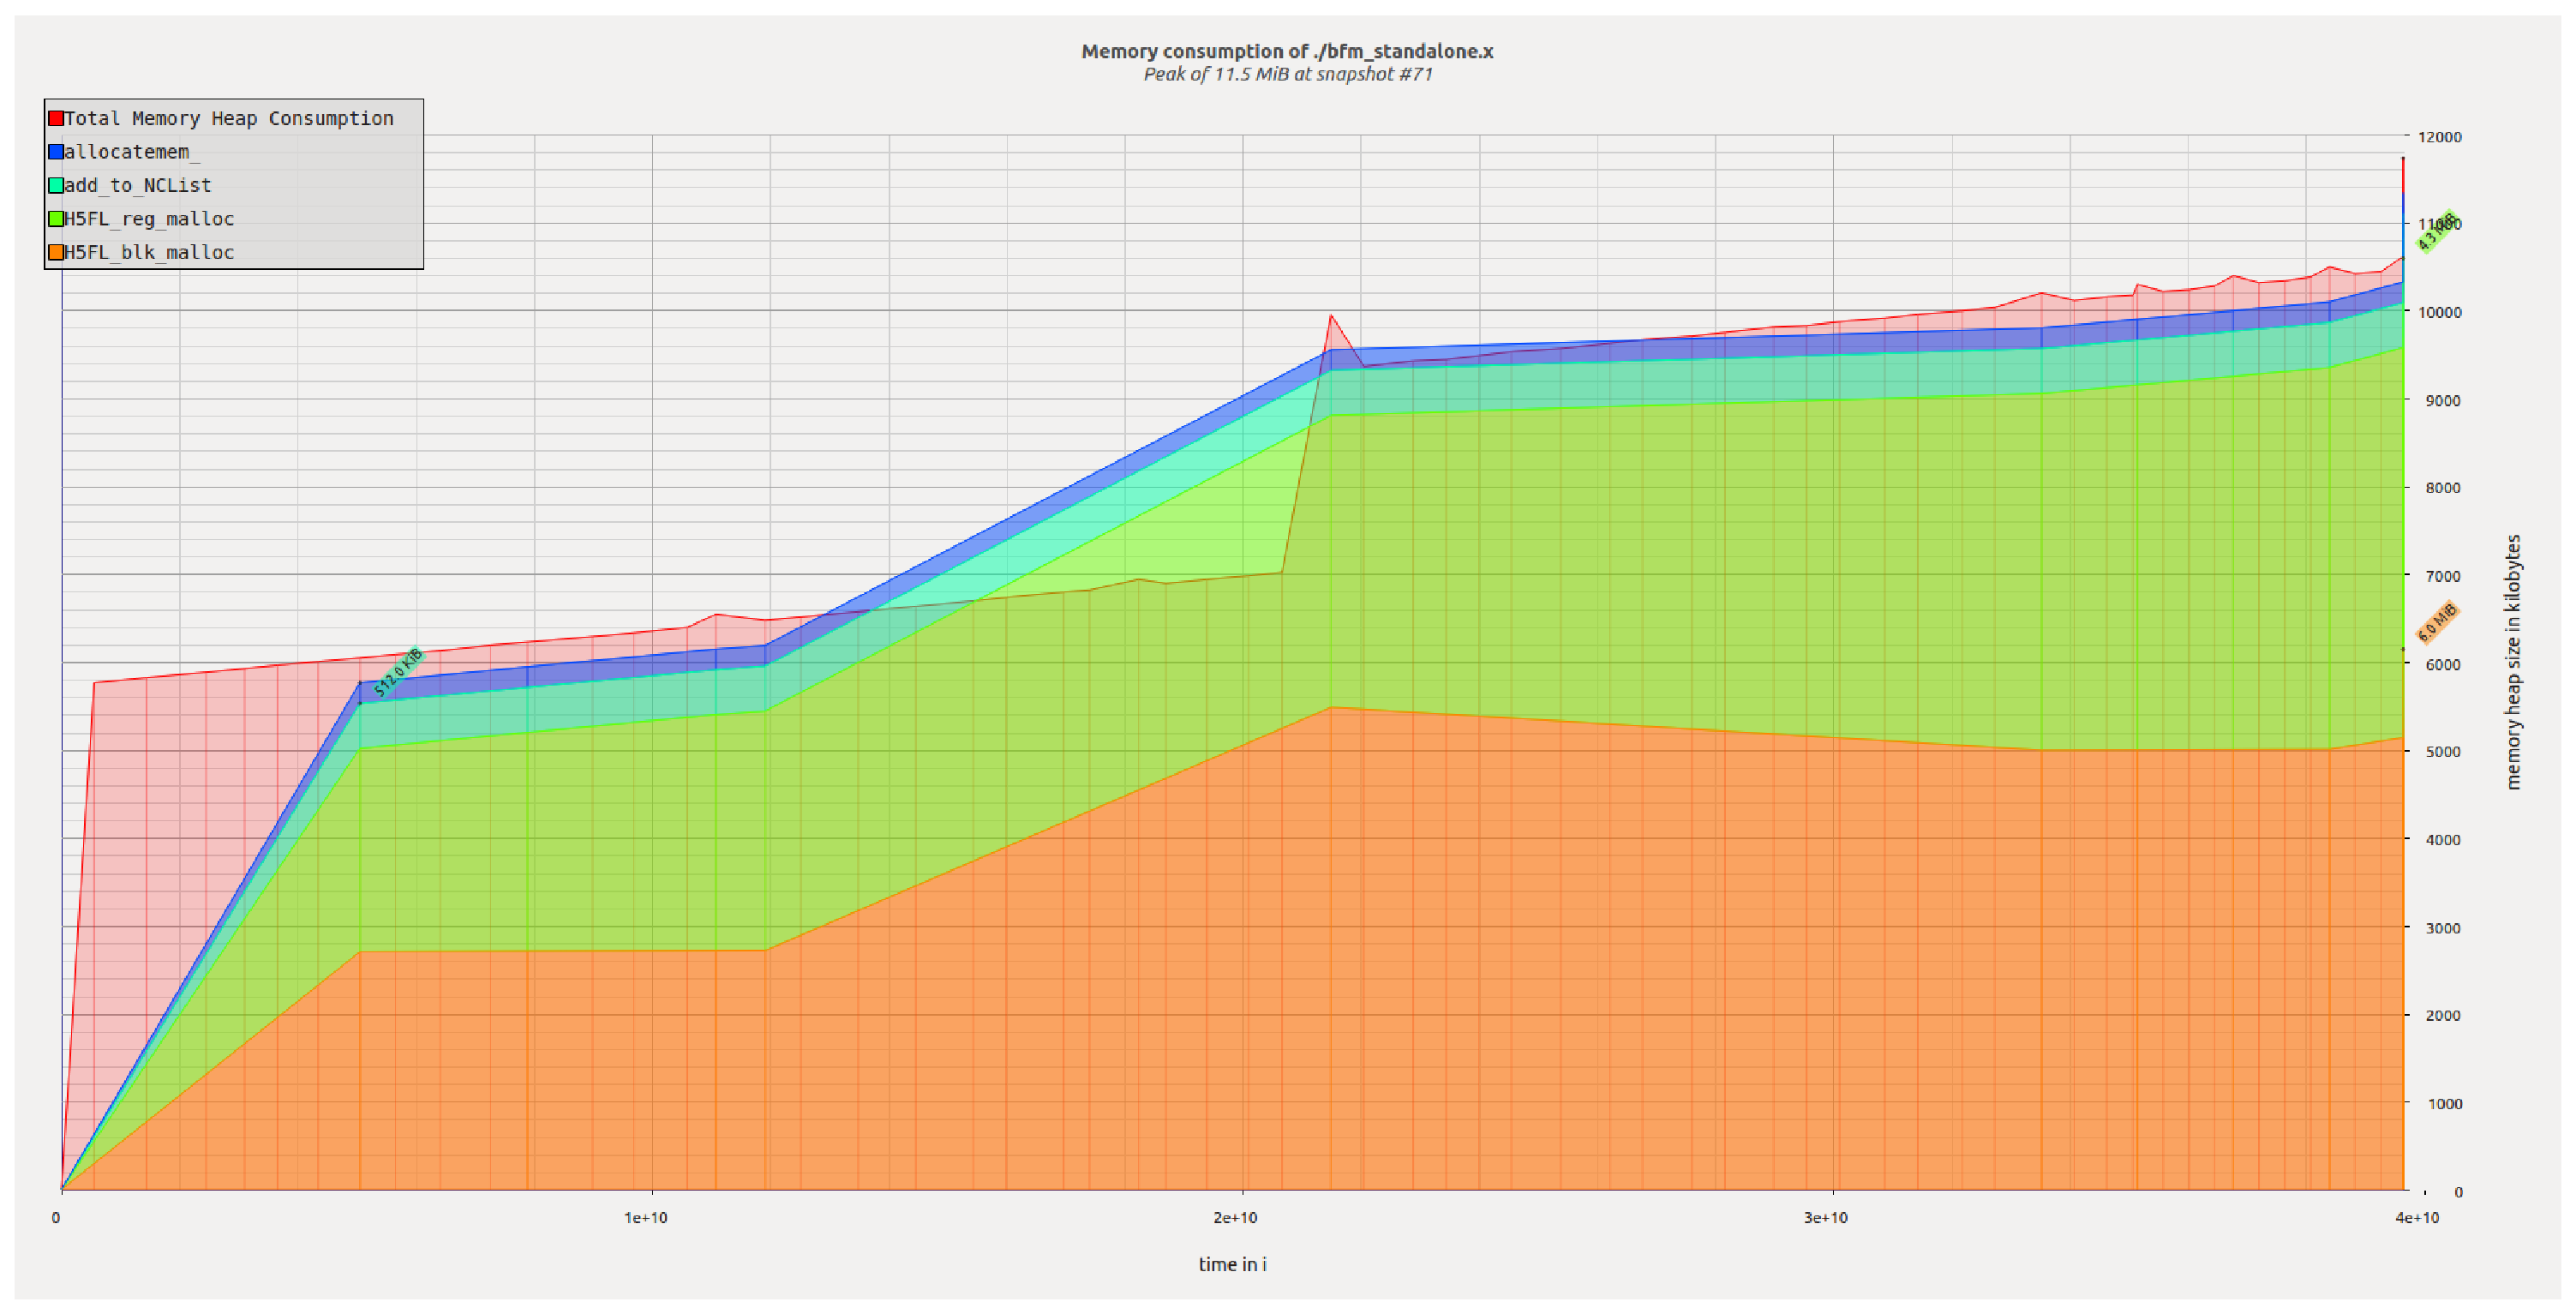
\includegraphics[width=\textwidth]{img/massif_std}
  \caption{Standalone Pelagic Memory Use Graph}
  \label{fig:massif_std}
\end{figure*}


\section{Gyre}\label{sec:gyre}
\subsection{Configuration}
\subsubsection{IFORT}
\begin{tabular}{|c|c|}
\hline
\hline
\rowcolor{LightCyan}
{\bf OPTION}   & {\bf VALUE} \\
\hline    
NAME     & test\_GYRE\_BFM \\                                                                       
\hline                                                                                              
ACTIVE   & A \\
\hline                                                                                              
PRESET   & GYRE\_BFM \\
\hline                                                                                               
RUN      & bsub \\
\hline                                                                                               
PROC     & '' \\
\hline                                                                                            
ARCH     & Ifort\_athena\_xios \\
\hline                                                                                            
RUNEXE   & '' \\
\hline                                                                                            
PAREXE   & '' \\
\hline                                                                                            
QUEUE    & 'poe\_long' \\
\hline                                                                                            
PRECMD   & module load HDF5/hdf5-1.8.11\_parallel \\
         & NETCDF/netcdf-4.3\_parallel \\
         & NETCDF/parallel-netcdf-1.3.1 \\
\hline                                                                                            
FORCING  & /work/ans040/FORCING/NEMO/*;/work/ans040/FORCING/BFM/* \\
\hline                                                                                            
PRERUN   & cp \$BFMDIR/tools/bfm\_test/configurations/PROFILING\_TESTS/pelagos\_cfg ./namelist\_cfg \\
\hline                                                                                            
COMPARE  & '' \\
\hline                                                                                            
VALGRIND & '' \\
\hline                                                                                            
\end{tabular}


\subsubsection{GFORTRAN}
\begin{tabular}{|c|c|}
\hline
\hline
\rowcolor{LightCyan}
{\bf OPTION}   & {\bf VALUE} \\
\hline    
NAME     & test\_GYRE\_BFM\_CI \\
\hline                                                                             
ACTIVE   & A \\
\hline                                                                             
PRESET   & GYRE\_BFM \\
\hline                                                                             
RUN      & bsub \\
\hline                                                                             
PROC     & '' \\
\hline                                                                             
ARCH     & ifort\_athena\_xios\_debug \\
\hline                                                                             
RUNEXE   & '' \\
\hline                                                                             
PAREXE   & '' \\
\hline                                                                             
QUEUE    & 'poe\_long' \\
\hline                                                                             
PRECMD   & module load HDF5/hdf5-1.8.11\_parallel \\
         & NETCDF/netcdf-4.3\_parallel \\
         & NETCDF/parallel-netcdf-1.3.1 \\
\hline                                                                             
FORCING  & '' \\
\hline                                                                             
PRERUN   & '' \\
\hline                                                                             
COMPARE  & '/users/home/ans040/dev/repo/bfm/tools/bfm\_test/tmp/test\_GYRE\_BFM' \\
\hline                                                                             
VALGRIND & valgrind --tool=callgrind --collect-jumps=yes --dump-instr=yes \\
\hline        
\end{tabular}


\subsubsection{VALGRIND}
\begin{tabular}{|c|c|c|}
\hline
\hline
\rowcolor{LightCyan}
{\bf OPTION}   & {\bf VALUE IFORT} & {\bf VALUE GFORTRAN}\\
\hline        
NAME     & test\_GYRE\_BFM\_MI & test\_GYRE\_BFM\_MG \\
\hline                                                                                                
ACTIVE   & A & A \\
\hline                                                                                                
PRESET   & GYRE\_BFM & GYRE\_BFM \\
\hline                                                                                             
RUN      & bsub & bsub \\
\hline                                                                                             
PROC     & '' & '' \\
\hline                                                                                             
ARCH     & ifort\_athena\_xios\_debug & gfortran\_athena\_xios\_debug \\
\hline                                                                                                
RUNEXE   & '' & '' \\
\hline                                                                                                
PAREXE   & '' & '' \\
\hline                                                                                                
QUEUE    & 'poe\_long' & 'poe\_long' \\
\hline                                                                                                
PRECMD   & \footnotemark[1] & \footnotemark[2] \\
\hline
FORCING  & '' &  '' \\
\hline     
PRERUN   & '' &  '' \\
\hline                         
COMPARE  & \footnotemark[3] & \footnotemark[4] \\
\hline    
VALGRIND & \footnotemark[5] & \footnotemark[6] \\
\hline        
\end{tabular}

\footnotetext[1]{module load HDF5/hdf5-1.8.11\_parallel NETCDF/netcdf-4.3\_parallel NETCDF/parallel-netcdf-1.3.1}
\footnotetext[2]{export NETCDF=/users/home/ans040/local; export LD\_LIBRARY\_PATH=/users/home/ans040/local/lib:\$LD\_LIBRARY\_PATH}
\footnotetext[3]{'/users/home/ans040/dev/repo/bfm/tools/bfm\_test/tmp/test\_GYRE\_BFM'}
\footnotetext[4]{'/users/home/ans040/dev/repo/bfm/tools/bfm\_test/tmp/test\_GYRE\_BFM'}
\footnotetext[5]{valgrind --tool=massif --stacks=yes}
\footnotetext[6]{valgrind --tool=massif --run-libc-freeres=no --stacks=yes}


\subsection{Result}

\begin{figure*}
  \centering
  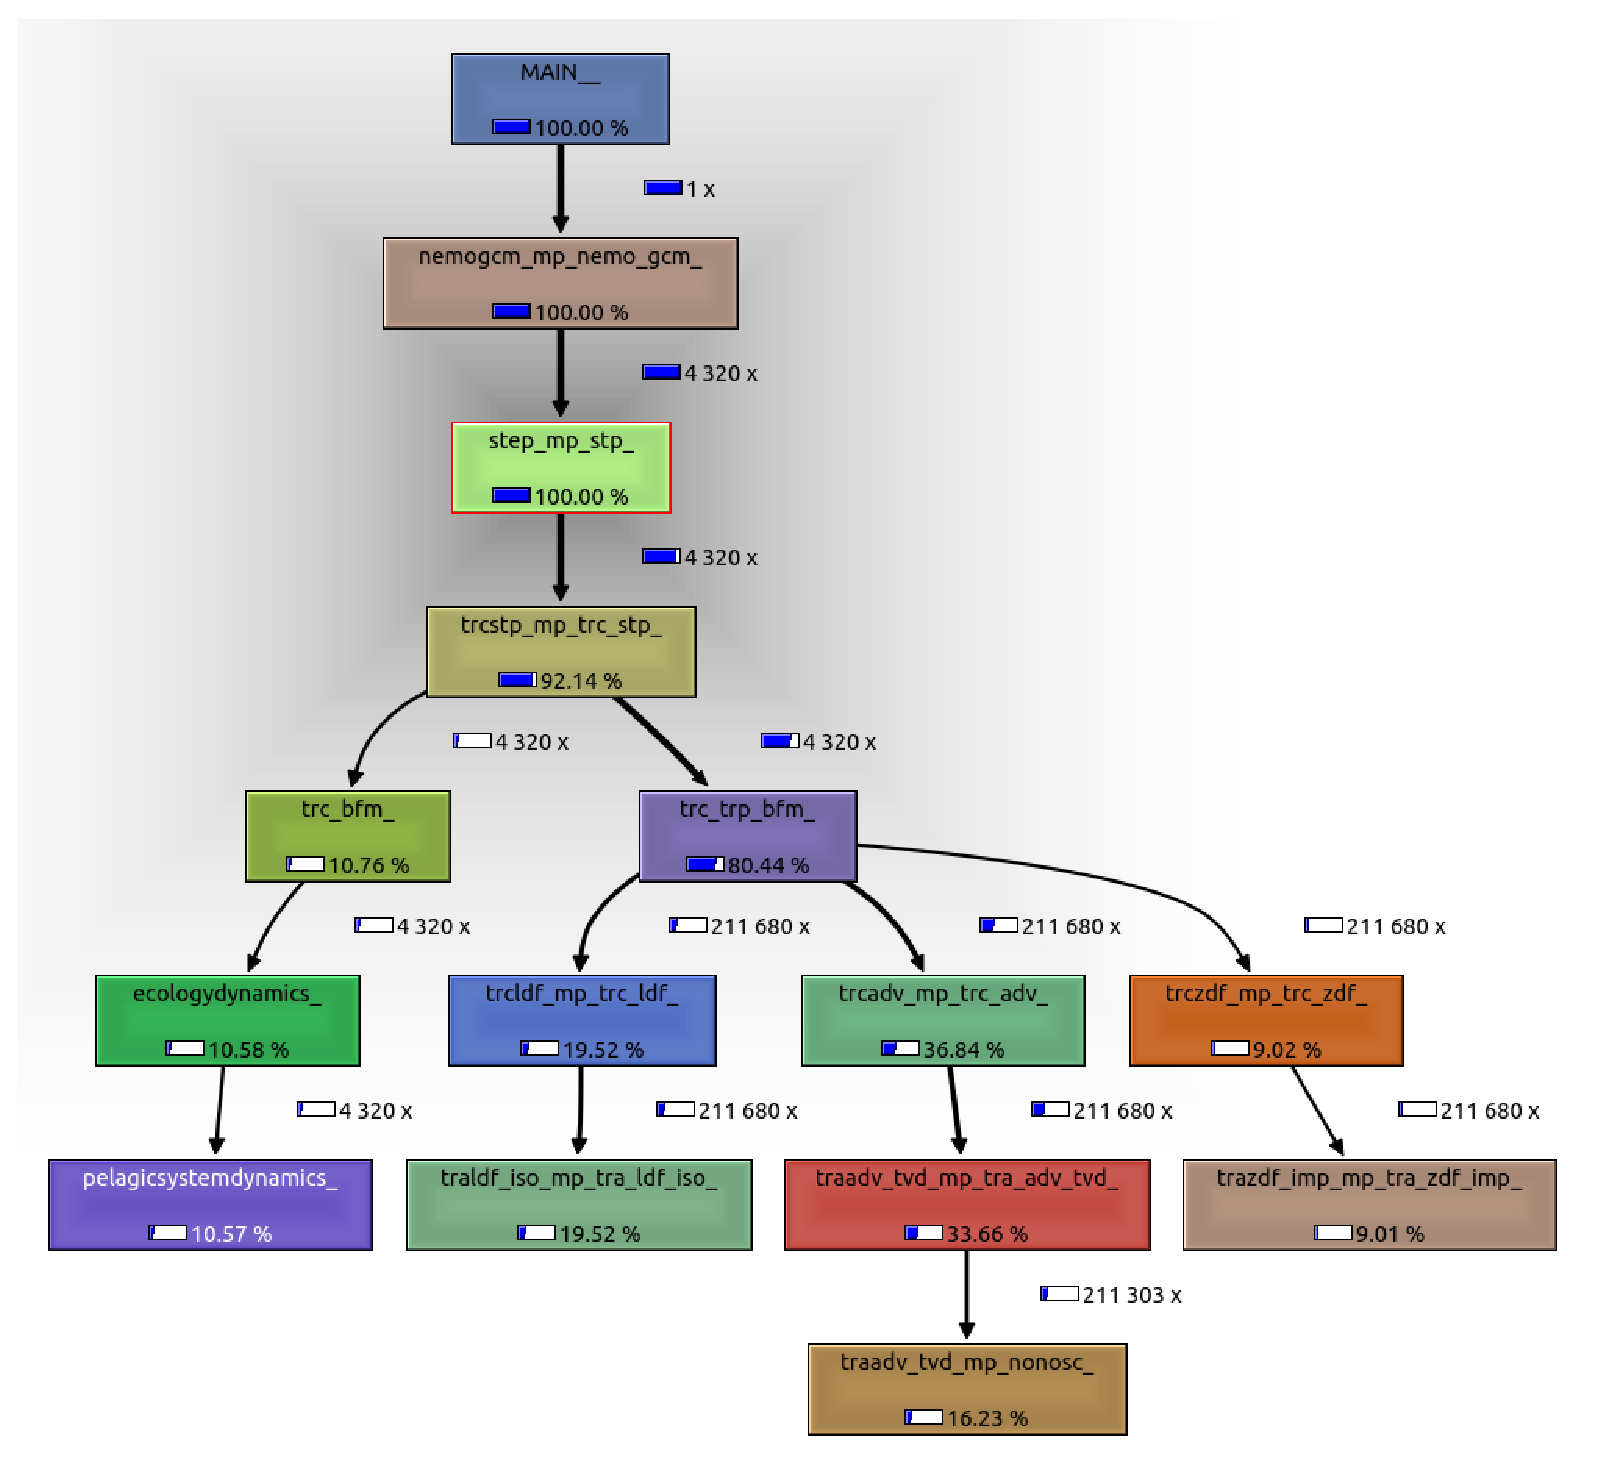
\includegraphics[width=\textwidth]{img/callgrind_gyre}
  \caption{Gyre Call Graph}
  \label{fig:callgrind_std}
\end{figure*}

\clearpage

\begin{figure*}
  \centering
  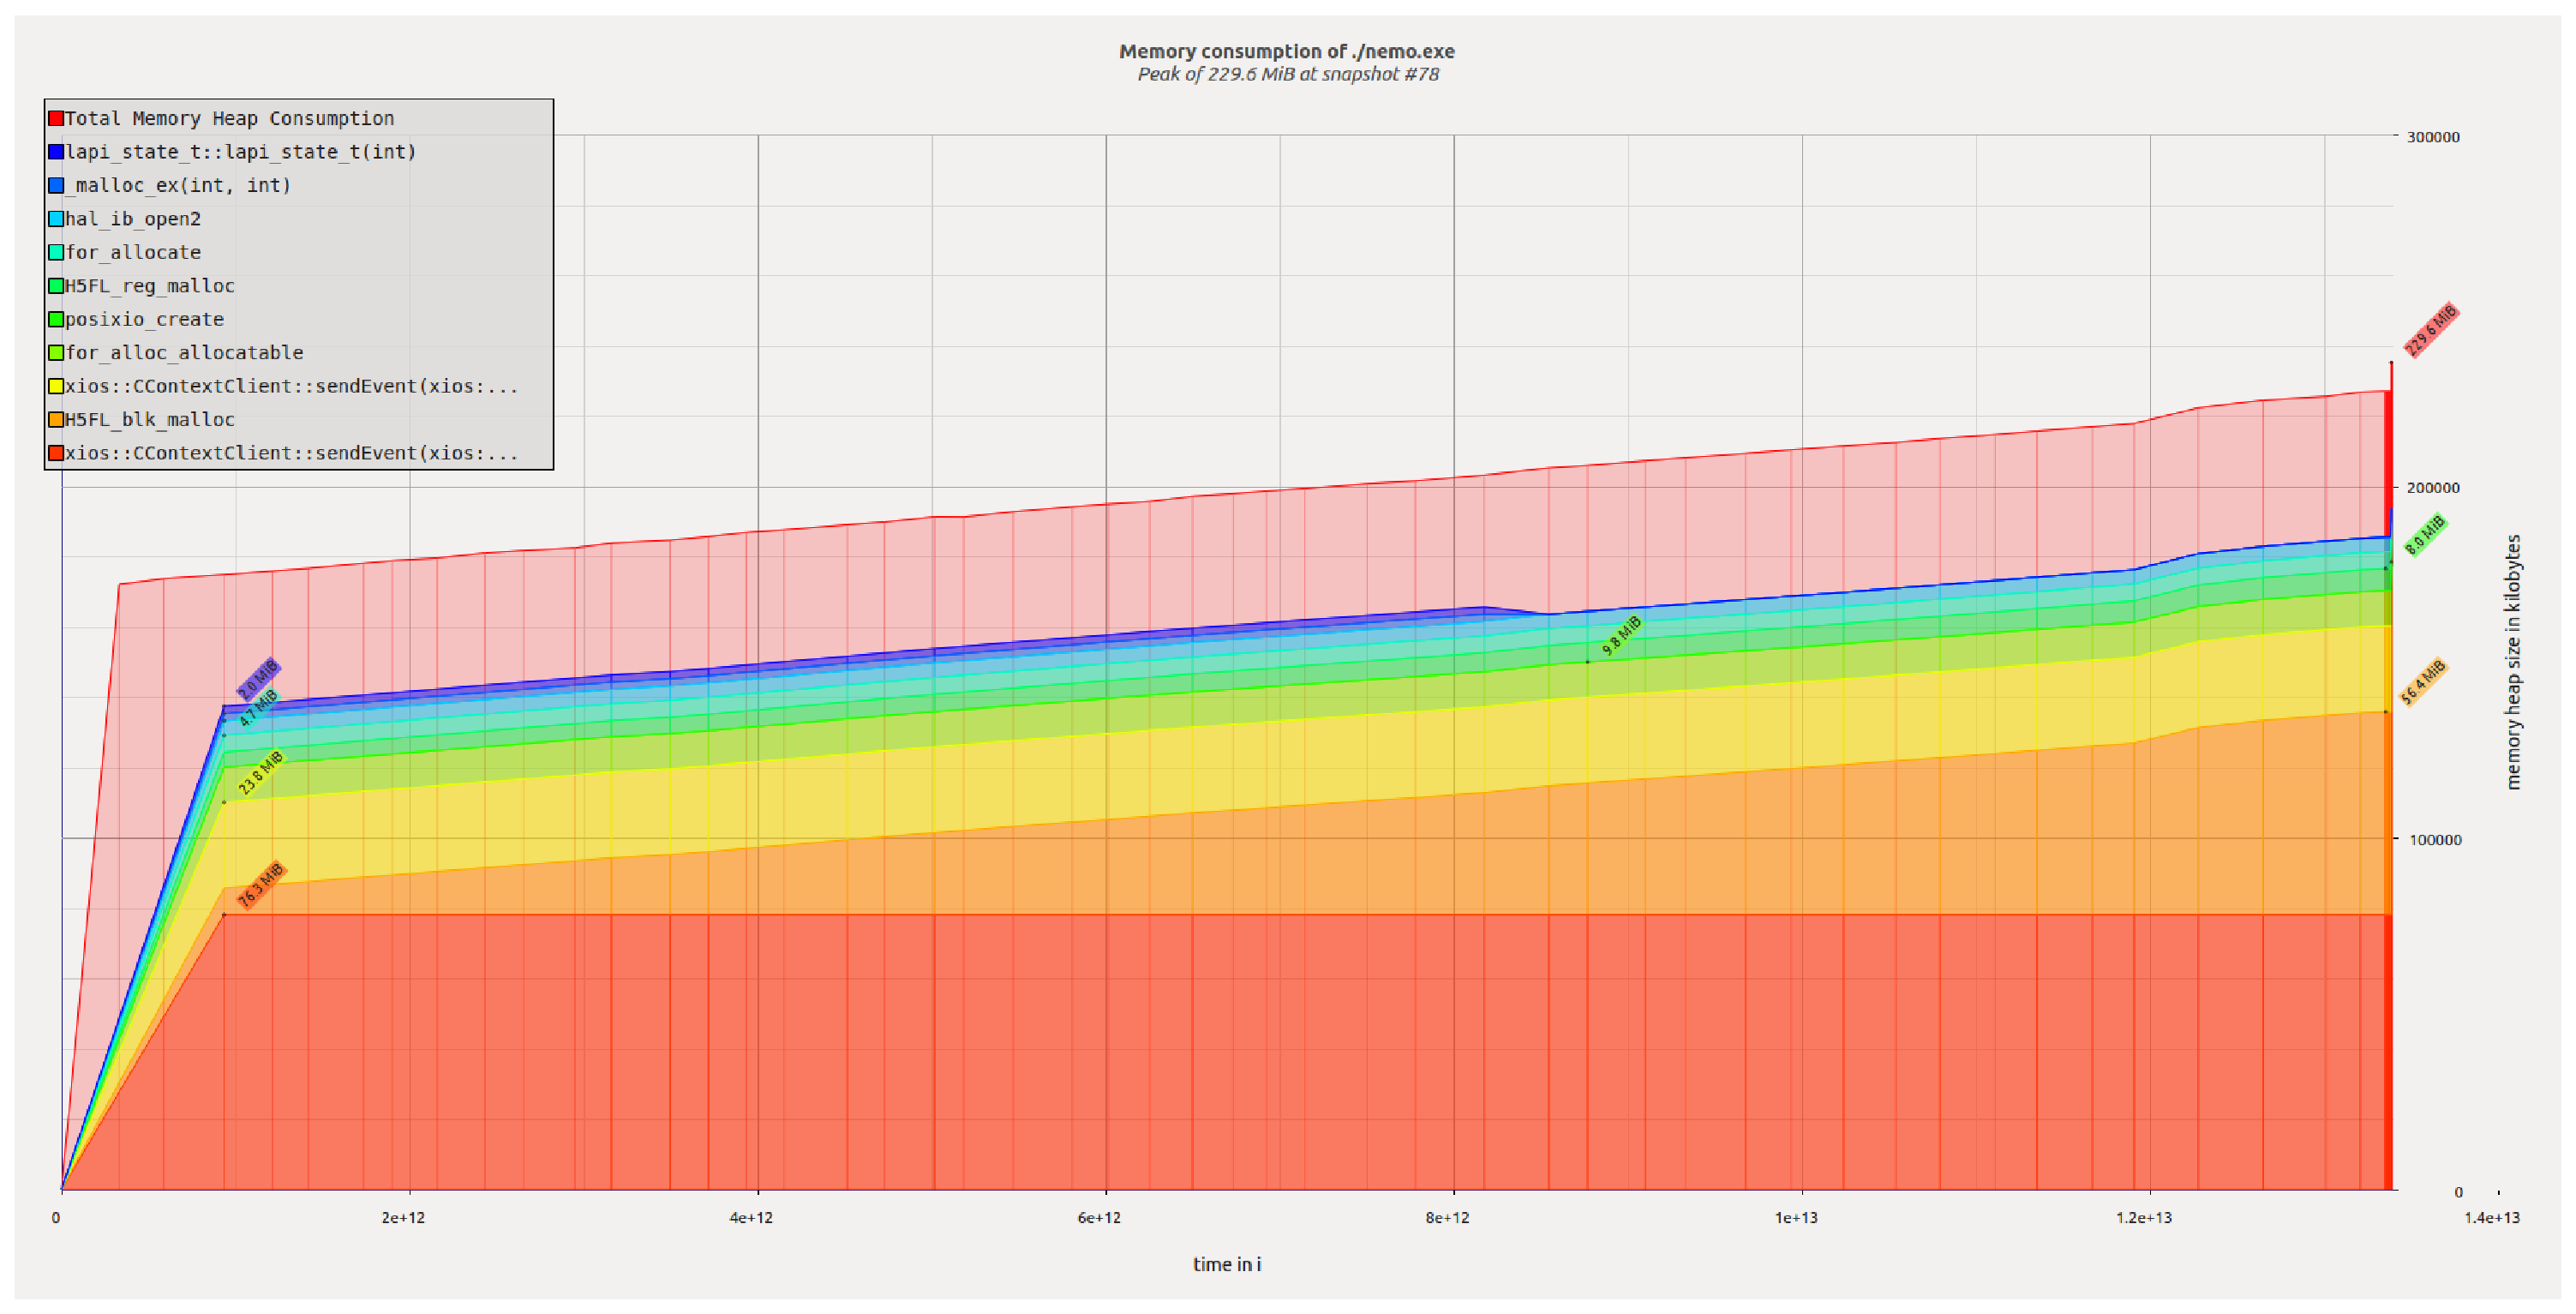
\includegraphics[width=\textwidth]{img/massif_gyre_mi}
  \caption{Gyre with Ifortran compiler Memory Use Graph}
  \label{fig:massif_std}
\end{figure*}

\begin{figure*}
  \centering
  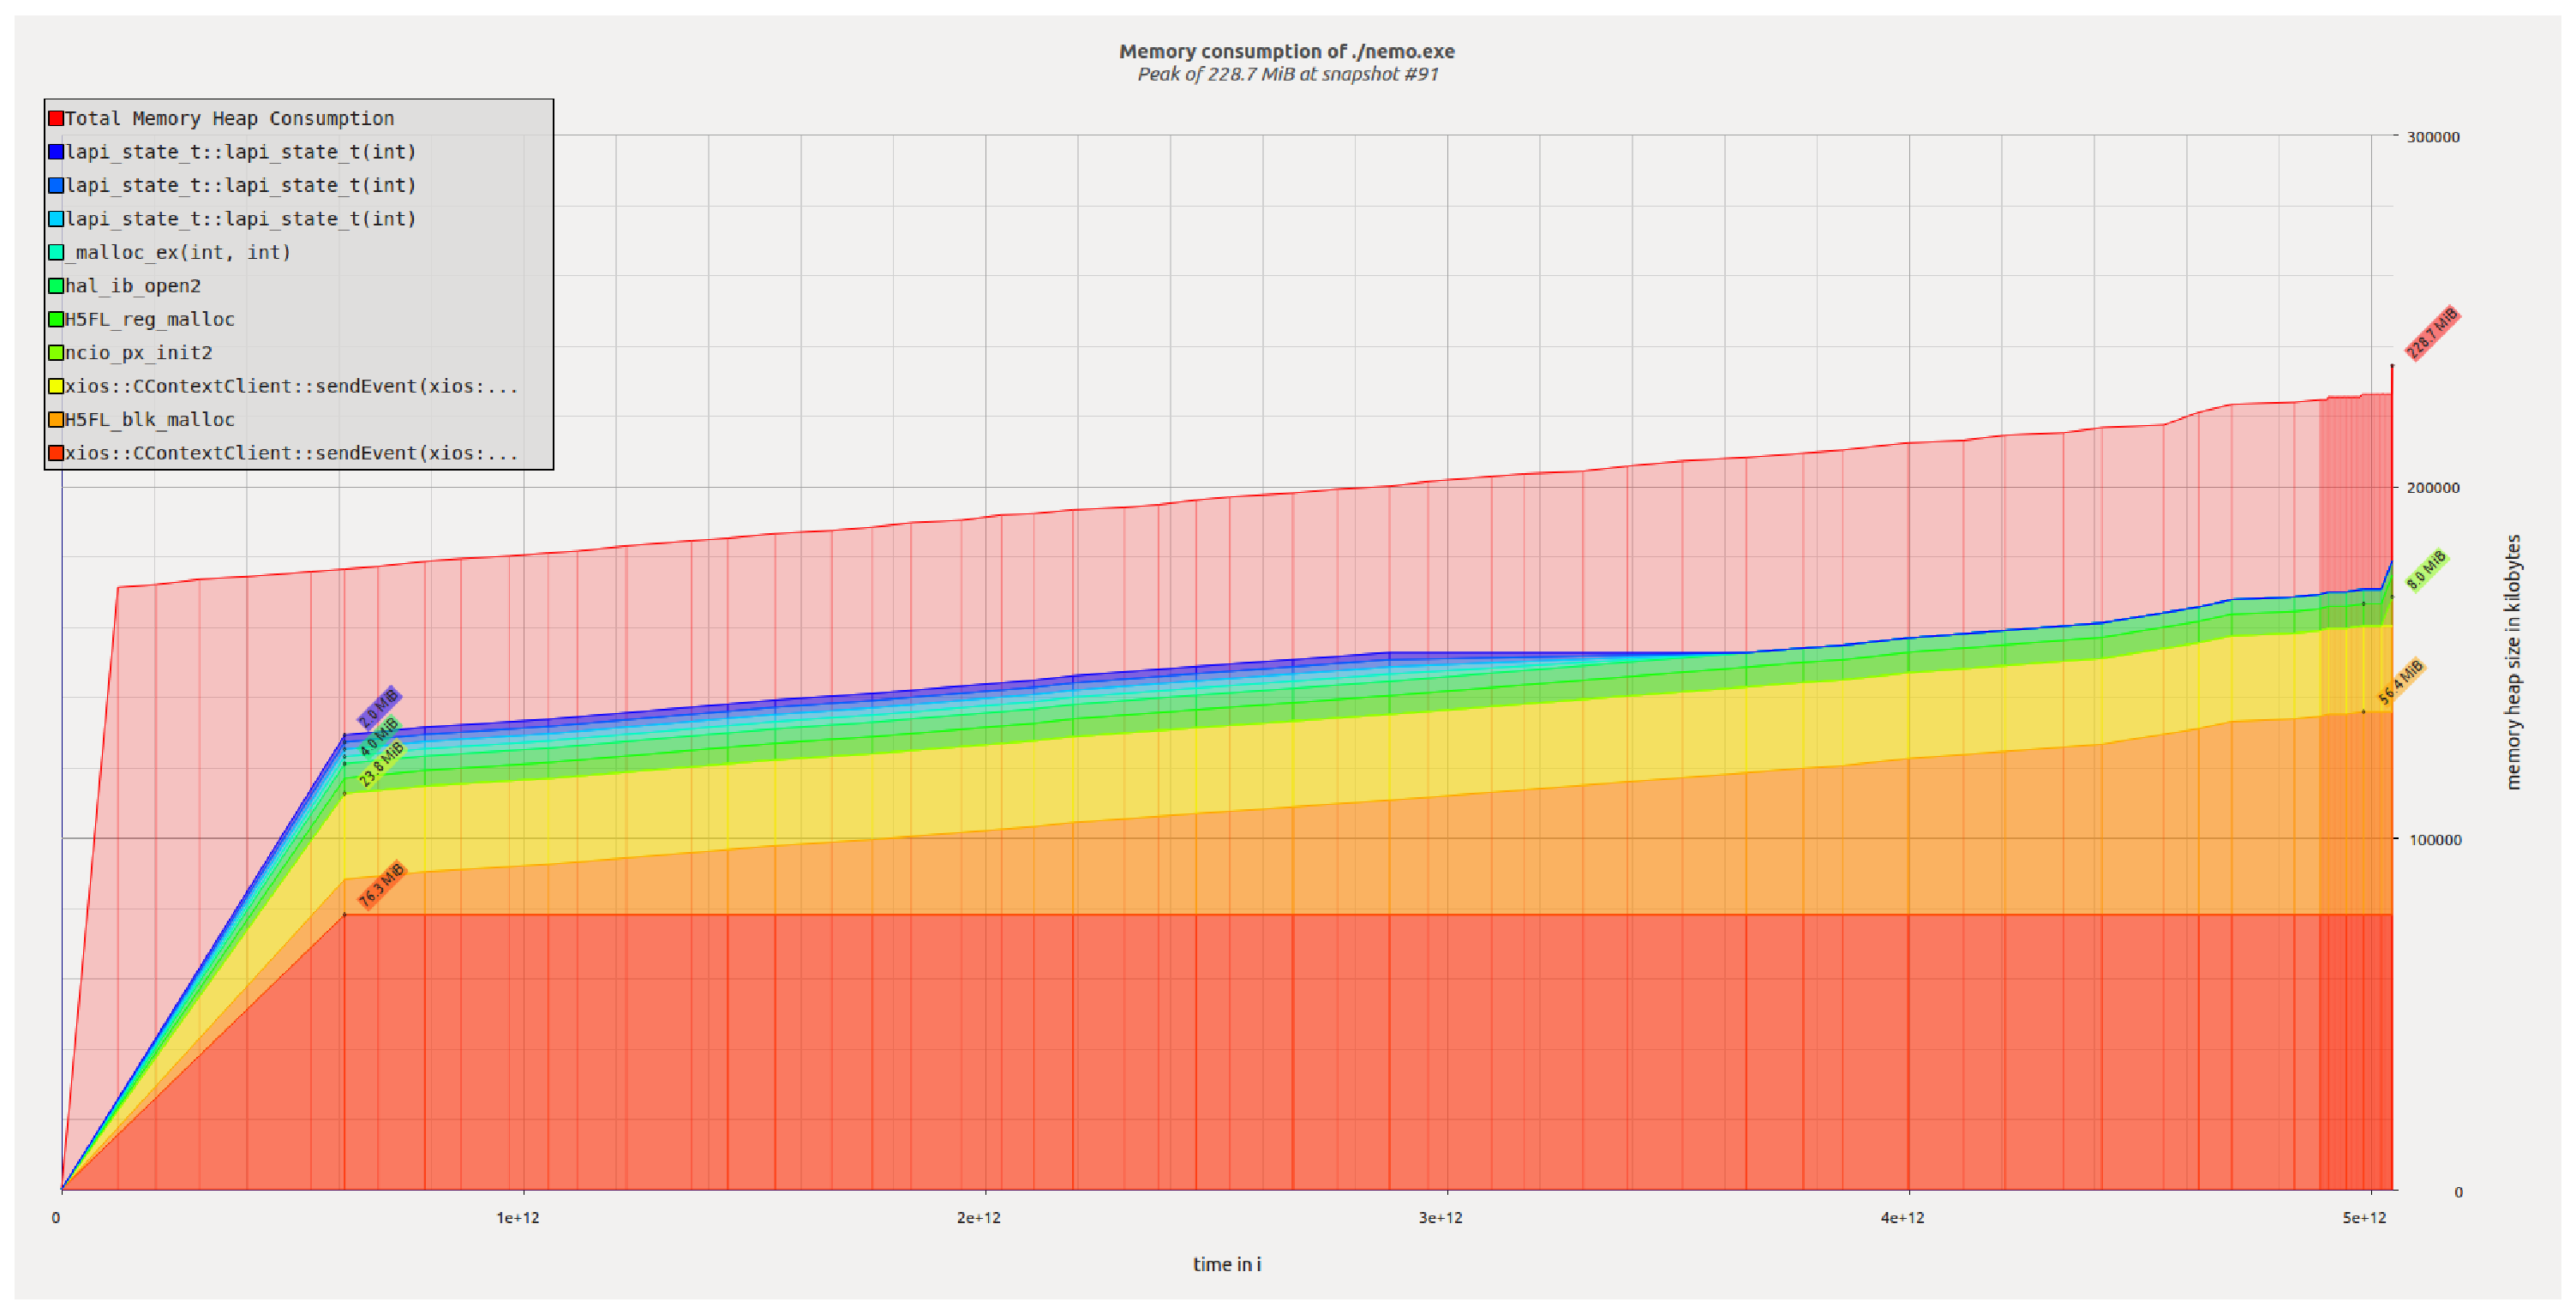
\includegraphics[width=\textwidth]{img/massif_gyre_mg}
  \caption{Gyre with Gfortran compiler Memory Use Graph}
  \label{fig:massif_std}
\end{figure*}
